\section{Begriffsklärung}
Das Wort \glqq Drohne\grqq\ ist eng mit dem militärischen Einsatz von unbemannten Flugkörpern verknüpft und wird mit dem Einsatz als tötende Waffe assoziiert. Es besteht keine Verknüpfung zu der Beschreibung eines unbewaffneten, vorwiegend für Freizeitaktivitäten und zivilen Einsatz eingesetzten Fluggerätes\cite{Buch_Engl}.


\ac{UAV} sind unbemannte Fluggeräte, welche entweder von Bodenpersonal gesteuert werden oder vollkommen autark fliegen. Es gibt sie in den verschiedensten Ausführungen, von einigen Zentimetern Größe(Revell Nano Quad) bis hin zu der Größe eines Jumbojets(Boeing Condor). Es gibt autark fliegende Hubschrauber, Flugzeuge und mehrrotorige \ac{UAV}. Selbst die von Wernher von Braun entwickelte \ac{V2} wird als ein selbständig fliegendes Objekt bezeichnet. Sie war  mit Mechanismen ausgestattet, die eine korrekte Zielführung sicherstellten und zur Not den Kurs automatisch anpassen konnten \cite{V2}.

\section{Allgemeines zu \acs{UAV}}
\subsection{Geschichte}

1849 gab es erste Aufzeichnungen von \ac{UAV}. Es waren mit Bomben bestückte Heißluftballons von österreichischen Entwicklern. Die Ballons wurden über einen Kupferdraht ferngezündet (Siehe Abbildung:   \ref{ballonbombs}). Charles Perley entwickelte dieses Verfahren im Jahre 1863 weiter, indem er Bomben per Zeitzünder abwarf \cite{baloonbombs}.

Im ersten Weltkrieg wurde von Elmer Sperry und Peter Cooper Hewitt das  Hewitt-Sperry Automatic Airplane (genannt: Flying Bomb, siehe Abbildung: \ref{Flying Bomb}) entwickelt. Dieses Flugzeug war in der Lage einen vordefinierten Kurs zu halten.
Zu einem bestimmten Zeitpunkt wurden geladene Torpedos ausgelöst. Sie konnten durch gyroskopische Stabilisierer die Richtung halten.\cite{flyingbomb}

In den 30iger Jahren entwickelte Reginald Denny funkgesteuerte Flugzeuge zum Training der US Army. 1935 entwarf er seine \ac{RP-1}, die er in den folgenden Jahren bis zur RP-5 weiterentwickelte. Die \ac{RP-1} war dafür ausgelegt, die Luftabwehrschützen der US Army zu trainieren, indem die \ac{RP-1} als Zielscheibe genutzt wurde. Sie war das erste, in Masse gefertigte, \ac{UAV}.\cite{RP-1}

1941 wurde in das \ac{UAV} namens \textit{Culver Cadet} eine Kamera eingebaut, die auf einem Bildschirm eines zweiten bemannten Flugzeuges zu sehen war, wodurch Einsätze einen viel größeren Radius haben konnten.

In den 60er Jahren rückte das Thema \emph{Überwachung von anderen Staaten} zunehmend in die Interessen der amerikanischen Verteidigungspolitik. Es wurde ein Langstreckenaufklärer vom Typ Ryan Model 147A (Codename: Fire Fly, siehe Abbildung \ref{fire fly}) entwickelt. Dieser konnte über Entfernungen von bis zu 1930 Kilometern operieren. Sie wurde eingesetzt um Länder wie Vietnam, Kuba, China und Nordkorea auszuspionieren.\cite{FireFly}

Der derzeitige Stand der Technik wird bei den Militär- \ac{UAV} durch die Northrop Grumman RQ-4(Global Hawk) definiert. Es kann in großen Höhen (bis zu 20 km) operieren. Die Flugzeit wird mit über 34 Std. angegeben(siehe Abbildung:\ref{global hawk}) \cite{rq-4}.


\subsection{Einsatzgebiete}
Es gibt die verschiedensten Einsatzgebiete unbemannter Luftfahrzeuge. Zum Einen gibt es den militärischen Sektor, indem \acp{UAV} dafür eingesetzt werden, um Aufklärungsflüge in extremen Höhen und großen Reichweiten zu ermöglichen. Die Northrop Grumman RQ-4 (Global Hawk)(siehe Abbildung:\ref{global hawk}) agiert zum Beispiel in einer Höhe von bis zu 20 Kilometer und hat einen Einsatzradius von 7500 Kilometern.

\begin{wrapfigure}{r}{0.5\textwidth}
  \begin{center}
    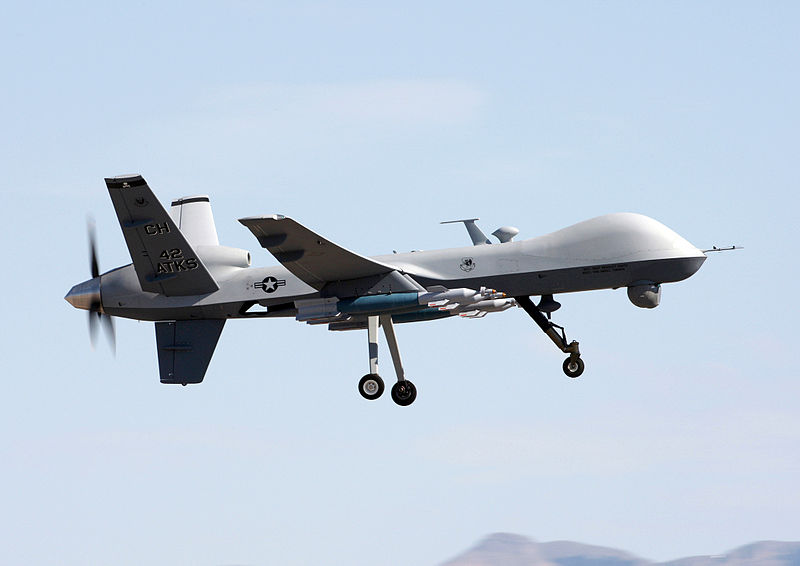
\includegraphics[width=0.48\textwidth]{img/reaper.jpg}
  \end{center}
  \caption{Eine MQ-9 Reaper bei einem Trainingseinsatz.©gemeinfrei}
  \label{reaper}
\end{wrapfigure}

Dies ermöglicht es eine Aufklärungsmission zu erfüllen wie zum Beispiel ein \ac{UAV} über Peking(VR China), gestartet und gesteuert aus Deutschland. Kontrolliert wird der Global Hawk von einem Kontrollzentrum aus, gestützt von modernster Satellitenkommunikation.
Militärische Drohnen können auch Bomben und Raketen aufnehmen. Der erstmalige Einsatz bewaffneter Drohnen ereignete sich am 27. Oktober 2007. Die \ac{MQ-9}(dt.Sensenmann,siehe Abbildung: \ref{reaper}) kann mit zwei 500 Pfund Bomben und vier Hellfire Raketen ausgestattet werden. Sie wurde schon in einigen Einsätzen in Krisengebieten für Luftschläge eingesetzt \cite{MQ-9}.

Zum Anderen werden \acp{UAV} im privaten Sektor für vielfältige Aufgaben eingesetzt. In der Agrarwirtschaft werden sie z.B. zur Detektion von Wildvieh in Anbauflächen eingesetzt (siehe Abbildung \ref{rehkitz}). 
Mittels hochsensiblen Wärmebildkameras kann so ein Zusammenstoß mit Erntemaschinen vermieden werden. Mit diversen Hochleistungskameras und Sensoren kann z.B. der Stickstoffgehalt aus hyperspektralen Bilddaten erkannt werden\cite{workshop_agrar}. Um Pflanzenschutzmittel gezielt in den Bewuchs einzubringen nutzt werden Aufnahmnen von \ac{UAV} genutzt, um Unkrautballungen auf z.B. Ackerflächen zu identifizieren\cite{unkraut}. Selbst das Ausbringen von Pflanzenschutzmitteln auf Ackerland ist mit \ac{UAV} durchaus möglich\cite{holzapfel}.\parfillskip=0pt
 In der Forschung werden \ac{UAV} zur Beobachtung von, für den Menschen unzugänglichen bzw. zu gefährlichen Orten benutzt.\par So kann z.B. radioaktiv verseuchtes Gebiet oder ein aktiver Vulkan untersucht werden ohne das Menschenleben gefährdet werden. Des Weiteren werden sie für Inspektionen an schwer zugänglichen Stellen von Hochspannungsmasten und Brückenpfeilern benutzt. In der Vergangenheit mussten diese Tätigkeiten von einem erfahrenen Helikopterpiloten durchgeführt werden. Diese Arbeiten waren sehr kostenintensiv und gefährlich.


\begin{wrapfigure}{r}{0.6\textwidth}
  \begin{center}
    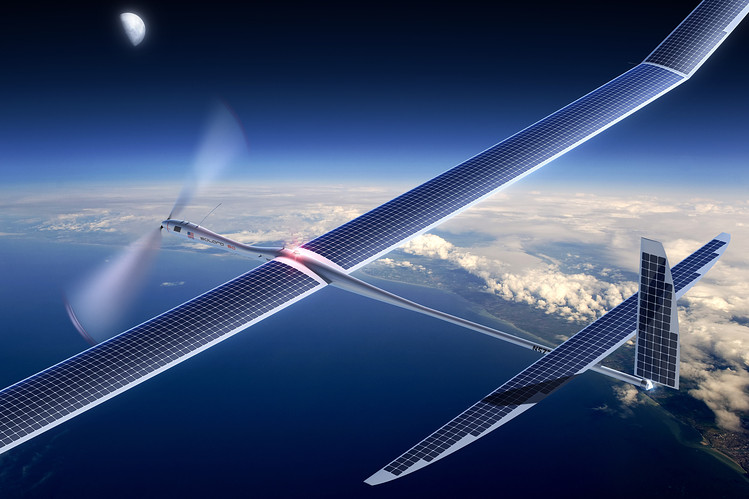
\includegraphics[width=0.5\textwidth]{img/solara50.jpg}
  \end{center}
  \caption{Eine Solara 50.©Titan Aerospace}
  \label{solara}
\end{wrapfigure}

Sie dienen als Relaisstationen für Daten bzw. Kommunikation jeglicher Art. So können \acp{UAV} in großen Höhen Funksignale empfangen und an Empfänger, die durch die Erdkrümmung oder funkstörender Objekte nicht direkt erreicht werden können, weitergeben. Erst kürzlich kaufte der Internetkonzern \textit{Google} den Solardrohnenhersteller \textit{Titan Aerospace}. Die daraus entwickelten Drohnen vom Typ Solara 50 (siehe Abbildung nebenstehend \ref{solara}) sollen eng verbunden mit Googles Projekt Loon als Relaisstationen Internet in die entlegensten Orte auf der Welt bringen. Es soll ein Gürtel aus Solara 50 und gasgefüllten Ballons in einer Höhe von 18 bzw. 32 Kilometern um die Erde gelegt werden. Die Solara 50 kann bis zu 5 Jahre ohne Landung eigenständig in der Luft bleiben \cite{loon}\cite{loon2}.
Wo früher noch aufwendige Luftaufnahmen per Helikopter notwendig waren, werden heute \ac{UAV} mit hochauflösenden Filmkameras ausgerüstet und fliegen äußerst flexibel über Drehsets.
Feuerwehren nutzen die Luftaufklärung zur Ermittlung von Brandherden(siehe dazu:\href{http://youtu.be/_yngOox3oJ4}{Youtube - Luftaufnahme Großbrand}).
Für Städte, Firmen und Tourismusagenturen ist es eine kostengünstige Möglichkeit Luftaufnahmen der Region/ Unternehmung in Imagefilme einzubinden. Auch die Deutsche Telekom nutzt \ac{UAV} um gegen Kupferdiebstahl vorzugehen. Es ist geplant per \ac{UAV} oberirdische Kupferleitungen mit eine Lösung zu bestreichen. Diese Flüssigkeit leuchtet unter \acs{UV-Licht} gelbgrün. Identifiziert wird auf zwei Wegen, zum einen besteht diese künstliche \glqq \acs{DNA}\grqq\ aus verschiedenen Basen. Deren typische Zusammenstellung ermöglicht ein klares zuordnen bei einem Kabeldiebstahl. Der zweite Weg geht über 400 Mikromillimeter kleine Nickelplättchen in der Flüssigkeit. Auf diesen Plättchen sind Identifkationscodes eingraviert die unter einem Mikroskop abgelesen werden können\cite{telekom}.
